\chapter{Complex Problem Set}
\begin{abox}
	Practise Set-1
\end{abox}
\begin{enumerate}[label=\color{ocre}\textbf{\arabic*.}]
	\item The value of the integral $\int_{C} d z z^{2} e^{z}$, where $C$ is an open contour in the complex $z$-plane as shown in the figure below, is:
	{\exyear{NET/JRF(JUNE-2011)}}
	\begin{figure}[H]
		\centering
		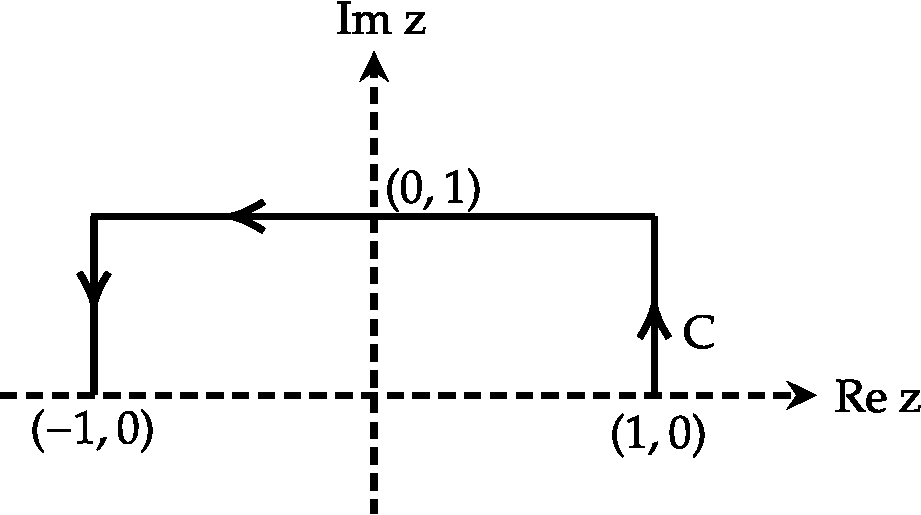
\includegraphics[height=5cm,width=9cm]{diagram-20211005-crop}
	\end{figure}
	\begin{tasks}(4)
		\task[\textbf{A.}] $\frac{5}{e}+e$
		\task[\textbf{B.}] $e-\frac{5}{e}$
		\task[\textbf{C.}] $\frac{5}{e}-e$
		\task[\textbf{D.}] $-\frac{5}{e}-e$
	\end{tasks}
	\begin{answer}
		\begin{align*}
		\intertext { If we complete the contour, then by Cauchy integral theorem }
		\int_{-1}^{1} d z z^{2} e^{z}+\int_{C} d z z^{2} e^{z}&=0 \Rightarrow \int_{C} d z z^{2} e^{z}=-\int_{-1}^{1} d z z^{2} e^{z}\\&=-\left[z^{2} e^{z}-2 z e^{2}+2 e^{2}\right]_{-1}^{1}=\frac{5}{e}-e
		\end{align*}
		So the correct answer is \textbf{Option (C)}
	\end{answer}
	\item Which of the following is an analytic function of the complex variable $z=x+i y$ in the domain $|z|<2 ?$
	{\exyear{NET/JRF(JUNE-2011)}}
	\begin{tasks}(2)
		\task[\textbf{A.}] $(3+x-i y)^{7}$
		\task[\textbf{B.}] $(1+x+i y)^{4}(7-x-i y)^{3}$
		\task[\textbf{C.}] $(1-x-i y)^{4}(7-x+i y)^{3}$
		\task[\textbf{D.}] $(x+i y-1)^{1 / 2}$
	\end{tasks}
	\begin{answer}
		Put $z=x+i y .$ If $\bar{z}=x-i y$ appears in any of the expressions then that expression is non-analytic. For option (D) we have a branch point singularity as the power is $\frac{1}{2}$ which is fractional. Hence only option (B) is analytic.\\\\
		So the correct answer is \textbf{Option (B)}
	\end{answer}
	\item The first few terms in the Laurent series for $\frac{1}{(z-1)(z-2)}$ in the region $1 \leq|z| \leq 2$ and around $z=1$ is
	{\exyear{NET/JRF(JUNE-2012)}}
	\begin{tasks}(1)
		\task[\textbf{A.}] $\frac{1}{2}\left[1+z+z^{2}+\ldots\right]\left[1+\frac{z}{2}+\frac{z^{2}}{4}+\frac{z^{3}}{8}+\ldots .\right]$
		\task[\textbf{B.}] $\frac{1}{1-z}-z-(1-z)^{2}+(1-z)^{3}+\ldots .$
		\task[\textbf{C.}] $\frac{1}{\mathrm{z}^{2}}\left[1+\frac{1}{\mathrm{z}}+\frac{1}{\mathrm{z}^{2}}+\ldots .\right]\left[1+\frac{2}{\mathrm{z}}+\frac{4}{\mathrm{z}^{2}}+\ldots . .\right]$
		\task[\textbf{D.}]  $2(z-1)+5(z-1)^{2}+7(z-1)^{3}+\ldots$
	\end{tasks}
	\begin{answer}
		\begin{align*}
		\frac{1}{(z-1)(z-2)}&=\frac{1}{z-2}-\frac{1}{z-1}=\frac{1}{1-z}+\frac{1}{(z-1)-1}\\&=\frac{1}{1-z}-(1+(1-z))^{-1}\\
		&=\frac{1}{1-z}-\left[1+(1-z)+\frac{(-1)(-2)}{2 !}(1-z)^{2}+\frac{(-1)(-2)(-3)}{3 !}(1-z)^{3} \ldots\right]\\
		&=\frac{1}{1-z}-\left[z+(1-z)^{2}-(1-z)^{3}+\ldots . .\right]
		\end{align*}
		So the correct answer is \textbf{Option (B)}
	\end{answer}
	\item Let $u(x, y)=x+\frac{1}{2}\left(x^{2}-y^{2}\right)$ be the real part of analytic function $f(z)$ of the complex variable $z=x+i y$. The imaginary part of $f(z)$ is
	{\exyear{NET/JRF(JUNE-2012)}}
	\begin{tasks}(4)
		\task[\textbf{A.}] $y+x y$
		\task[\textbf{B.}] $x y$
		\task[\textbf{C.}] $y$
		\task[\textbf{D.}] $y^{2}-x^{2}$
	\end{tasks}
	\begin{answer}
		\begin{align*}
		u(x, y)&=x+\frac{1}{2}\left(x^{2}-y^{2}\right), v(x, y)=?\\
		\text{Check }\frac{\partial u}{\partial x}&=\frac{\partial v}{\partial y}\text{ and } \frac{\partial u}{\partial y}=-\frac{\partial v}{\partial x}\\
		\Rightarrow \frac{\partial u}{\partial x}&=\frac{\partial v}{\partial y}, \quad \frac{\partial v}{\partial y}=1+x, \\ v&=y+x y+f(x)\\
		\frac{\partial u}{\partial y}&=-\frac{\partial v}{\partial x} \Rightarrow \frac{\partial v}{\partial x}=+y, \\ v&=y x+f(y)\\
		y+x y+f(x)&=y x+f(y)\\
		\text{If }f(x)&=0\quad \quad
		f(y)=y\\
		v&=x y+y
		\end{align*}
		So the correct answer is \textbf{Option (A)}
	\end{answer}
	\item The value of the integral $\int_{C} \frac{z^{3} d z}{\left(z^{2}-5 z+6\right)}$, where $C$ is a closed contour defined by the equation $2|z|-5=0$, traversed in the anti-clockwise direction, is
	{\exyear{NET/JRF(DEC-2012)}}
	\begin{tasks}(4)
		\task[\textbf{A.}] $-16 \pi i$
		\task[\textbf{B.}] $16 \pi \mathrm{i}$
		\task[\textbf{C.}] $8 \pi i$
		\task[\textbf{D.}] $2 \pi i$
	\end{tasks}
	\begin{answer}
		\begin{align*}
		z^{2}-5 z+6&=0 \Rightarrow z^{2}-2 z-3 z+6\\&=0 \Rightarrow z(z-2)-3(z-2)=0 \Rightarrow z=3,2\\
		2|z|&=5 \Rightarrow|z|=2.5,\text{ only 2 will be inside.}\\
		\text{Residue }&=\left.(z-2) \frac{z^{3}}{(z-3)(z-2)}\right|_{z=2}=\frac{8}{2-3}\\&=-8 \Rightarrow \int \frac{z^{3} d z}{z^{2}-5 z+6}=2 \pi i(-8)=-16 \pi i
		\end{align*}
		So the correct answer is \textbf{Option (A)}
	\end{answer}
	\item  With $z=x+i y$, which of the following functions $f(x, y)$ is NOT a (complex) analytic function of $z$ ?
	{\exyear{NET/JRF(JUNE-2013)}}
	\begin{tasks}(1)
		\task[\textbf{A.}] $f(x, y)=(x+i y-8)^{3}\left(4+x^{2}-y^{2}+2 i x y\right)^{7}$
		\task[\textbf{B.}] $f(x, y)=(x+i y)^{7}(1-x-i y)^{3}$
		\task[\textbf{C.}] $f(x, y)=\left(x^{2}-y^{2}+2 i x y-3\right)^{5}$
		\task[\textbf{D.}] $f(x, y)=(1-x+i y)^{4}(2+x+i y)^{6}$
	\end{tasks}
	\begin{answer}
		\begin{align*}
		f(x, y)&=(1-x+i y)^{4}(2+x+i y)^{6}\\&=\{1-(x-i y)\}^{4}(2+x+i y)^{6}\\
		\text{Due to present of }\bar{z}&=(x-i y)
		\end{align*}
		So the correct answer is \textbf{Option (D)}
	\end{answer}
	\item  Which of the following functions cannot be the real part of a complex analytic function of $z=x+i y ?$
	{\exyear{NET/JRF(DEC-2013)}}
	\begin{tasks}(4)
		\task[\textbf{A.}] $x^{2} y$
		\task[\textbf{B.}]  $x^{2}-y^{2}$
		\task[\textbf{C.}] $x^{3}-3 x y^{2}$
		\task[\textbf{D.}] $3 x^{2} y-y-y^{3}$
	\end{tasks}
	\begin{answer}
		\begin{align*}
		\intertext{ Let $x^{2} y$ be real part of a complex function. Use Milne Thomson's method to write analytic complex function. The real part of that function should be (1) but that is not the case. So this cannot be real part of an analytic function. Also,}
		z^{2}&=(x+i y)^{2}=x^{2}-y^{2}+2 i x y,\text{ Real part option (2)}\\
		z^{3}&=(x+i y)^{3}=x^{3}-i y^{3}+3 i x y(x+i y)\\
		&=x^{3}-i y^{3}+3 i x^{2} y-3 x y^{2},\text{ Real part option (3)}
		\end{align*}
		So the correct answer is \textbf{Option (A)}
	\end{answer}
	\item  Given that the integral $\int_{0}^{\infty} \frac{d x}{y^{2}+x^{2}}=\frac{\pi}{2 y}$, the value of $\int_{0}^{\infty} \frac{d x}{\left(y^{2}+x^{2}\right)^{2}}$ is
	{\exyear{NET/JRF(DEC-2013)}}
	\begin{tasks}(4)
		\task[\textbf{A.}] $\frac{\pi}{y^{3}}$
		\task[\textbf{B.}] $\frac{\pi}{4 y^{3}}$
		\task[\textbf{C.}]  $\frac{\pi}{8 y^{3}}$
		\task[\textbf{D.}] $\frac{\pi}{2 y^{3}}$
	\end{tasks}
	\begin{answer}
		\begin{align*}
		\int_{0}^{\infty} \frac{d x}{\left(y^{2}+x^{2}\right)^{2}}&=\frac{1}{2} \int_{-\infty}^{\infty} \frac{d x}{\left(y^{2}+x^{2}\right)^{2}},\text{ pole is of }2^{\text {nd }}\text{ order at }x=i y,\text{ residue }=1 /\left(4 i y^{3}\right)\\
		\text{Integral }&=\left(\frac{1}{2}\right)(2 \pi i) \frac{1}{4 i y^{3}}=\frac{\pi}{\left(4 y^{3}\right)}
		\end{align*}
	\end{answer}
	\item If $C$ is the contour defined by $|z|=\frac{1}{2}$, the value of the integral
	$$
	\oint_{C} \frac{d z}{\sin ^{2} z}
	$$
	is
	{\exyear{NET/JRF(JUNE-2014)}}
	\begin{tasks}(4)
		\task[\textbf{A.}] $\infty$
		\task[\textbf{B.}] $2 \pi i$
		\task[\textbf{C.}] 0
		\task[\textbf{D.}] $\pi i$
	\end{tasks}
	\begin{answer}
		\begin{align*}
		f(z)&=\frac{1}{\sin ^{2} z} \quad\left(|z|=\frac{1}{2}\right)\\
		\sin z&=z-\frac{z^{3}}{\lfloor 3}+\frac{z^{5}}{\lfloor 5} \ldots . \Rightarrow \frac{1}{\sin ^{2} z}=\frac{1}{\left(z-\frac{z^{3}}{\frac{3}{3}}+\frac{z^{5}}{5} \cdots\right)^{2}}\\
		\Rightarrow \frac{1}{\sin ^{2} z}&=\frac{1}{z^{2}}\left[1-\frac{z^{2}}{\lfloor 3}+\frac{z^{4}}{\lfloor 5} \ldots .\right]^{-2} \Rightarrow \oint_{C} \frac{d z}{\sin ^{2} z}=0
		\end{align*}
		So the correct answer is \textbf{Option (C)}
	\end{answer}
	\item The principal value of the integral $\int_{-\infty}^{\infty} \frac{\sin (2 x)}{x^{3}} d x$ is
	{\exyear{NET/JRF(DEC-2014)}}
	\begin{tasks}(4)
		\task[\textbf{A.}] $-2 \pi$
		\task[\textbf{B.}]  $-\pi$
		\task[\textbf{C.}] $\pi$
		\task[\textbf{D.}]  $2 \pi$
	\end{tasks}
	\begin{answer}
		\begin{align*}
		\text{Let }f(z)&=\frac{e^{i 2 z}}{z^{3}}\\
		\lim _{2 \rightarrow 0}(z-0)^{3} f(z)&=\lim _{z \rightarrow 0}(z-0)^{3} \frac{e^{i 2 z}}{z^{3}}\\&=1(\text{ finite and }\neq 0) \Rightarrow z=0 \text{is pole of order 3} .\\
		\text{Residue }R&=\frac{1}{2 !} \lim _{z \rightarrow 0} \frac{d^{2}}{d z^{2}}\left[(z-0)^{3} \frac{e^{i 2 z}}{z^{3}}\right]=-2\\
		\Rightarrow \int_{-\infty}^{\infty} f(x) d x&=\pi i \Sigma R=\pi i(-2)=-2 \pi i \Rightarrow \operatorname{Im} .\text{ Part }\\&=-2 \pi \Rightarrow \int_{-\infty}^{\infty} f(x) d x=-2 \pi
		\end{align*}
		So the correct answer is \textbf{Option (A)}
	\end{answer}
	\item The Laurent series expansion of the function $f(z)=e^{2}+e^{1 / 2}$ about $z=0$ is given by
	{\exyear{NET/JRF(DEC-2014)}}
	\begin{tasks}(2)
		\task[\textbf{A.}] $\sum_{n=-\infty}^{\infty} \frac{z^{n}}{n !}$ for all $|z|<\infty$
		\task[\textbf{B.}] $\sum_{n=0}^{\infty}\left(z^{n}+\frac{1}{z^{n}}\right) \frac{1}{n !}$ only if $0<|z|<1$
		\task[\textbf{C.}] $\sum_{n=0}^{\infty}\left(z^{n}+\frac{1}{z^{n}}\right) \frac{1}{n !}$ for all $0<|z|<\infty$
		\task[\textbf{D.}]  $\sum_{n=-\infty}^{\infty} \frac{z^{n}}{n !}$ only if $|z|<1$
	\end{tasks}
	\begin{answer}
		\begin{align*}
		e^{z}&=\left(1+z+\frac{z^{2}}{2 !}+\ldots\right)=\sum_{n=0}^{\infty} \frac{z^{n}}{n !}\text{ and }e^{1 / z}\\&=1+\frac{1}{z}+\frac{1}{2 !} \frac{1}{z^{2}}+\ldots .=\sum_{n=0}^{\infty} \frac{1}{z^{n} n !}\\
		\Rightarrow f(z)&=\left(e^{z}+e^{1 / 2}\right)=\sum_{n=0}^{\infty}\left(z^{n}+\frac{1}{z^{n}}\right) \frac{1}{n !},\text{ for all }0<|z|<\infty
		\end{align*}
		So the correct answer is \textbf{Option (C)}
	\end{answer}
	\item Consider the function $f(z)=\frac{1}{z} \ln (1-z)$ of a complex variable $z=r e^{i \theta}(r \geq 0, \quad-\infty<\theta<\infty)$. The singularities of $f(z)$ are as follows:
	{\exyear{NET/JRF(DEC-2014)}}
	\begin{tasks}(1)
		\task[\textbf{A.}]  Branch points at $z=1$ and $z=\infty$; and a pole at $z=0$ only for $0 \leq \theta<2 \pi$
		\task[\textbf{B.}] Branch points at $z=1$ and $z=\infty$; and a pole at $z=0$ for all $\theta$ other than $0 \leq \theta<2 \pi$
		\task[\textbf{C.}] Branch points at $z=1$ and $z=\infty$; and a pole at $z=0$ for all $\theta$
		\task[\textbf{D.}] Branch points at $z=0, z=1$ and $z=\infty$.
	\end{tasks}
	\begin{answer}
		\begin{align*}
		\text{For }f(z)&=\frac{1}{z} \ln (1-z)=\frac{1}{z}\left(-z-\frac{z^{2}}{2}-\frac{z^{3}}{3}-\ldots . .\right)\\&=-1-\frac{z}{2}-\frac{z^{2}}{3}-\ldots .
		\intertext{There is no principal part and when $z \rightarrow 0, f(z)=-1 .$ So there is removable singularity at $z=0$. Also $z=1$ and $z=\infty$ is Branch point.}
		\end{align*}
		None of the above is correct
	\end{answer}
	\item  The value of integral $\int_{-\infty}^{\infty} \frac{d x}{1+x^{4}}$
	{\exyear{NET/JRF(JUNE-2015)}}
	\begin{tasks}(4)
		\task[\textbf{A.}] $\frac{\pi}{\sqrt{2}}$
		\task[\textbf{B.}] $\frac{\pi}{2}$
		\task[\textbf{C.}] $\sqrt{2} \pi$
		\task[\textbf{D.}] $2 \pi$
	\end{tasks}
	\begin{answer}
		\begin{align*}
		\int_{-\infty}^{\infty} \frac{d z}{1+z^{4}} \quad \because|z|=R\\
		\text{Now, pole }z&=e^{(2 n+1) \frac{\pi}{4}}\\
		n&=0, \quad \Rightarrow z_{0}=e^{\frac{i \pi}{4}}=\frac{1}{\sqrt{2}}+i \frac{1}{\sqrt{2}}, n\\&=2 \Rightarrow z_{2}=\frac{-1}{\sqrt{2}}-i \frac{1}{\sqrt{2}}\\
		n&=1 \Rightarrow z_{1}=e^{\frac{i 3 \pi}{4}}=\frac{-1}{\sqrt{2}}+i \frac{1}{\sqrt{2}}, n\\&=3 \Rightarrow z_{3}=+\frac{1}{\sqrt{2}}-i \frac{1}{\sqrt{2}}
		\intertext{only $z_{0}$ and $z_{1}$ lies in contour}
		\text{i.e., residue at }\left(z=e^{\frac{i \pi}{4}}\right)&=\frac{1}{4}\left(-\frac{1}{\sqrt{2}}-i \frac{1}{\sqrt{2}}\right)\\
		\text{residue at }\left(z=e^{\frac{i 3 \pi}{4}}\right)&=\frac{1}{4}\left(\frac{1}{\sqrt{2}}-i \frac{1}{\sqrt{2}}\right)\\
		\text{now }\int_{-\infty}^{\infty} \frac{d x}{x^{4}+1}&=2 \pi i \Sigma \operatorname{Re} S=\frac{\pi}{\sqrt{2}}
		\end{align*}
		So the correct answer is \textbf{Option (A)}
	\end{answer}
	\item  The function $\frac{Z}{\sin \pi z^{2}}$ of a complex variable $z$ has
	{\exyear{NET/JRF(DEC-2015)}}
	\begin{tasks}(1)
		\task[\textbf{A.}] A simple pole at 0 and poles of order 2 at $\pm \sqrt{n}$ for $n=1,2,3 \ldots$
		\task[\textbf{B.}] A simple pole at 0 and poles of order 2 at $\pm \sqrt{n}$ and $\pm i \sqrt{n}$ for $n=1,2,3 \ldots$
		\task[\textbf{C.}] Poles of order 2 at $\pm \sqrt{n}, n=0,1,2,3 \ldots$
		\task[\textbf{D.}] Poles of order 2 at $\pm n, n=0,1,2,3 \ldots$
	\end{tasks}
	\begin{answer}
		\begin{align*}
		f(z)&=\frac{z}{\sin \pi z^{2}}=\frac{z}{\pi z^{2} \frac{\sin \pi z^{2}}{\pi z^{2}}}\\
		\text{	at }z&=0,\text{ it is a simple pole since,} \lim _{z \rightarrow 0} \frac{\sin \pi z^{2}}{\pi z^{2}}=1\\
		\text{Also, }\sin \pi z^{2}&=\sin n \pi \Rightarrow \pi \mathrm{z}^{2}\\&=\pm n \pi, z=\pm \sqrt{n}, \pm i \sqrt{n}\\
		\lim _{z \rightarrow \sqrt{n}}&(z-\sqrt{n})^{2} \cdot \frac{z}{\sin \pi z^{2}}, \text{exists. So its pole of order 2}
		\end{align*}
		So the correct answer is \textbf{Option (B)}
	\end{answer}
	\item The value of the contour integral $\frac{1}{2 \pi i} \oint_{C} \frac{e^{4 z}-1}{\cosh (z)-2 \sinh (z)} d z$ around the unit circle $C$ traversed in the anti-clockwise direction, is
	{\exyear{NET/JRF(JUNE-2016)}}
	\begin{tasks}(4)
		\task[\textbf{A.}] 0
		\task[\textbf{B.}] 2
		\task[\textbf{C.}] $\frac{-8}{\sqrt{3}}$
		\task[\textbf{D.}] $-\tanh \left(\frac{1}{2}\right)$
	\end{tasks}
	\begin{answer}
		\begin{align*}
		f(z)&=\frac{e^{4 z}-1}{\cosh z-2 \sinh z}=\frac{e^{4 z}-1}{\frac{e^{2}+e^{-z}}{2}-\left(e^{z}-e^{-z}\right)}\\&=\frac{e^{42}-1}{-\frac{e^{z}}{2}+\frac{3}{2} e^{-z}}\\
		\Rightarrow f(z)&=\frac{2 e^{2}\left(e^{4 z}-1\right)}{\left(3-e^{2 z}\right)}=\frac{2\left(e^{5 z}-e^{z}\right)}{\left(3-e^{2 z}\right)}\\
		\text{For pole at }z&=z_{0}, 3-e^{2 \xi_{0}}=0 \Rightarrow e^{2 z_{0}}\\&=3 \Rightarrow z_{0}=\frac{\ln 3}{2}
		\intertext{It has simple pole at $z_{0}$}
		\operatorname{Re}\left(z_{0}\right)&=\lim _{z \rightarrow z_{0}}\left(z-z_{0}\right) f(z)=\lim _{2 \rightarrow z_{0}}\left(z-z_{0}\right) \frac{2\left(e^{5 z}-e^{2}\right)}{3-e^{22}}\\
		&=\lim _{z \rightarrow z_{0}} \frac{\left(z-z_{0}\right) \times 2\left(5 e^{5 z}-e^{z}\right)+2\left(e^{5 z}-e^{z}\right) \times 1}{-2 e^{2 z}}\\&=-\left(\frac{e^{5 z_{0}}-e^{z_{0}}}{e^{2 z_{0}}}\right)\\
		&=-\left(\frac{(\sqrt{3})^{5}-\sqrt{3}}{3}\right)=-\left(\frac{9 \sqrt{3}-\sqrt{3}}{3}\right)=-\frac{8}{\sqrt{3}}\\
		\frac{1}{2 \pi i} \oint f(z) d z&=\frac{1}{2 \pi i} \times 2 \pi i \sum\text{ Residue } =-\frac{8}{\sqrt{3}}
		\end{align*}
		So the correct answer is \textbf{Option (C)}
	\end{answer}
	\item  Let $u(x, y)=e^{a x} \cos (b y)$ be the real part of a function $f(z)=u(x, y)+i v(x, y)$ of the complex variable $z=x+i y$, where $a, b$ are real constants and $a \neq 0 .$ The function $f(z)$ is complex analytic everywhere in the complex plane if and only if
	{\exyear{NET/JRF(JUNE-2017)}}
	\begin{tasks}(4)
		\task[\textbf{A.}] $b=0$
		\task[\textbf{B.}] $b=\pm a$
		\task[\textbf{C.}] $b=\pm 2 \pi a$
		\task[\textbf{D.}]  $b=a \pm 2 \pi$
	\end{tasks}
	\begin{answer}
		\begin{align*}
		\intertext{The function $f(z)$ will be analytic everywhere in the complex plane if and only if it satisfies the Cauchy Riemann equation in that region.}
		\Rightarrow \frac{\partial u}{\partial x}&=\frac{\partial v}{\partial y}\text{ and } \frac{\partial u}{\partial y}=-\frac{\partial v}{\partial x}\\
		\text{Hence }a e^{a x} \cos (b y)&=\frac{\partial v}{\partial y}\hspace{2cm}\text{(i)}\\
		\text{and }b e^{a x} \sin (b y)&=\frac{\partial v}{\partial x}\hspace{2cm}\text{(ii)}
		\intertext{From equation (i)}
		v(x, y)&=\frac{a e^{a x} \sin (b y)}{b}+c(y)\hspace{2cm}\text{(iii)}
		\intertext{Differentiating partially with $x$ gives}
		\frac{\partial v}{\partial x}&=\frac{a^{2} e^{a x} \sin (b y)}{b}\hspace{2cm}\text{(iv)}
		\intertext{From equation (iii) and (iv)}
		b e^{a x} \sin (b y)&=\frac{a^{2} e^{a x} \sin (b y)}{b}\\
		\Rightarrow b^{2}&=a^{2} \Rightarrow b=\pm a
		\end{align*}
		So the correct answer is \textbf{Option (B)}
	\end{answer}
	\item  The integral $\oint_{\Gamma} \frac{z e^{i \pi z / 2}}{z^{2}-1} d z$ along the closed contour $\Gamma$ shown in the figure is
	{\exyear{NET/JRF(JUNE-2017)}}
	\begin{figure}[H]
		\centering
		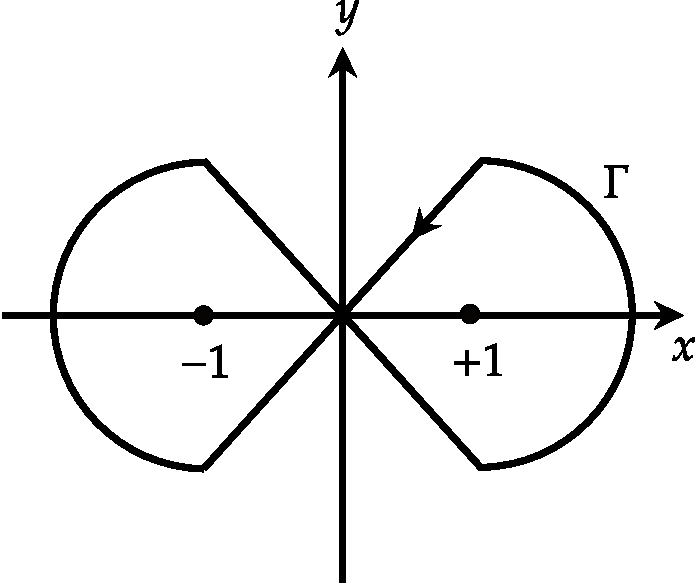
\includegraphics[height=4cm,width=5cm]{diagram-20211005(19)-crop}
	\end{figure}
	\begin{tasks}(4)
		\task[\textbf{A.}] 0
		\task[\textbf{B.}] $2 \pi$
		\task[\textbf{C.}] $-2 \pi$
		\task[\textbf{D.}] $4 \pi i$
	\end{tasks}
	\begin{answer}
		\begin{align*}
		f(z)&=\frac{z e^{i z \pi / 2}}{(z+1)(z-1)}\\
		\text{For }z&=+1\text{ anti-clockwise}\\
		I&=2 \pi i \lim _{z \rightarrow 1} \frac{z e^{i \pi z / 2}}{(z+1)}=\frac{2 \pi i}{2} e^{i \pi / 2}=\pi i e^{i \pi / 2}\\
		\text{For }z&=-1\\
		I&=-2 \pi i \lim _{z \rightarrow-1} \frac{z e^{i \pi z / 2}}{(z-1)}=-2 \pi i \times \frac{(-1) e^{-i \pi / 2}}{(-2)}=-\pi i e^{-i \pi / 2}\\
		\text{Integral }&=\pi i \frac{\left(e^{i \pi / 2}-e^{-i \pi / 2}\right)}{2 i} \times 2 i=2 \pi i^{2} \sin \frac{\pi}{2}=-2 \pi
		\end{align*}
		So the correct answer is \textbf{Option (C)}
	\end{answer}
	\item What is the value of $a$ for which $f(x, y)=2 x+3\left(x^{2}-y^{2}\right)+2 i(3 x y+a y)$ is an analytic function of complex variable $z=x+i y$
	{\exyear{NET/JRF(JUNE-2018)}}
	\begin{tasks}(4)
		\task[\textbf{A.}] 1
		\task[\textbf{B.}] 0
		\task[\textbf{C.}] 3
		\task[\textbf{D.}] 2
	\end{tasks}
	\begin{answer}
		\begin{align*}
		f(x, y)&=2 x+3\left(x^{2}-y^{2}\right)+2 i(3 x y+\alpha y)\\
		u&=2 x+3\left(x^{2}-y^{2}\right), v=2(3 x y+\alpha y)\\
		\text{C-R conditions: }u_{x}&=v_{y}, u_{y}=-v_{x}\\
		2+3(2 x)&=2(3 x+\alpha) \Rightarrow \alpha=1 \Rightarrow-6 y=-6 y
		\end{align*}
		So the correct answer is \textbf{Option (A)}
	\end{answer}
	\item  The value of the integral $\oint_{C} \frac{d z}{z} \frac{\tanh 2 z}{\sin \pi z}$, where $C$ is a circle of radius $\frac{\pi}{2}$, traversed counter-clockwise, with centre at $z=0$, is
	{\exyear{NET/JRF(DEC-2018)}}
	\begin{tasks}(4)
		\task[\textbf{A.}] 4
		\task[\textbf{B.}] $4 i$
		\task[\textbf{C.}] $2 i$
		\task[\textbf{D.}] 0
	\end{tasks}
	\begin{answer}$\left. \right. $
		\begin{figure}[H]
			\centering
			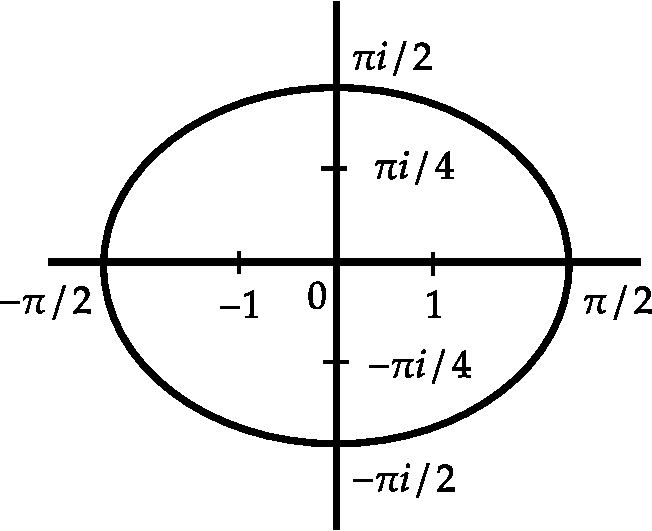
\includegraphics[height=4.5cm,width=5.5cm]{diagram-20211005(2)-crop}
		\end{figure}
		\begin{align*}
		&\oint_{C} \frac{d z}{z} \frac{\tanh 2 z}{\sin \pi z} d z\\
		z&=0,1,-1, \frac{\pi i}{4}, \frac{-\pi i}{4}\\
		f(z)&=\frac{2 z-\frac{1}{3}(2 z)^{3}+\frac{2}{15}(2 z)^{5} \ldots .}{z\left(\pi z-\frac{\pi^{3} z^{3}}{3 !}+\ldots\right)}\\
		\frac{2}{\pi z}&\left(1-\frac{1}{2} z^{2}+\ldots\right)\left(1-\frac{\pi^{2} z^{2}}{2 !}+\ldots\right)\\
		b_{1}&=\frac{2}{\pi}\\
		\text{As Re } z&=1, \frac{\tanh ^{2}}{-\pi}\text{ and }\operatorname{Re} z=-1, \frac{\tanh ^{2}}{-\pi}\\
		\operatorname{Re} z&=\frac{i \pi}{4}=-\frac{1}{\pi}\left(2 \operatorname{cosec} h \frac{\pi^{2}}{4}\right)\\
		\operatorname{Re} z&=\frac{-i \pi}{4}=-\frac{1}{\pi}\left(2 \operatorname{cosec} \mathrm{h} \frac{\pi^{2}}{4}\right)
		\intertext{$I=2 \pi i \Sigma R=4 i$ only when 0 lies inside, otherwise wrong question.}
		\end{align*}
		So the correct answer is \textbf{Option (B)}
	\end{answer}
	\item The integral $I=\int_{C} e^{z} d z$ is evaluated from the point $(-1,0)$ to $(1,0)$ along the contour $C$, which is an arc of the parabola $y=x^{2}-1$, as shown in the figure. The value of $I$ is
	{\exyear{NET/JRF(DEC-2018)}}
	\begin{figure}[H]
		\centering
		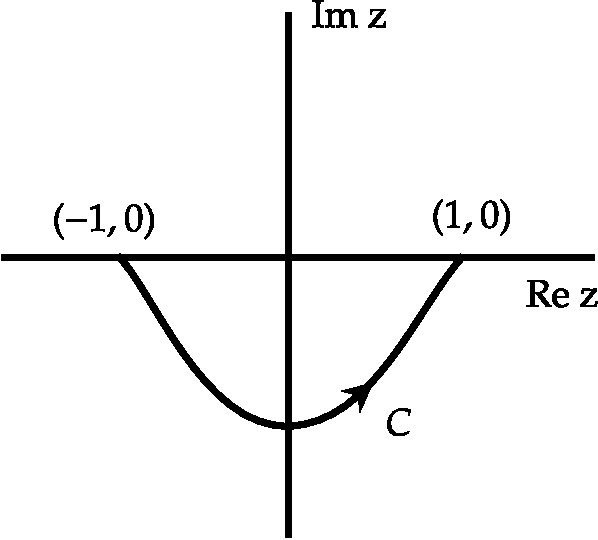
\includegraphics[height=4.5cm,width=5cm]{diagram-20211005(3)-crop}
	\end{figure}
	\begin{tasks}(4)
		\task[\textbf{A.}]  0
		\task[\textbf{B.}] $2 \sinh 1$
		\task[\textbf{C.}]  $e^{2 i} \sinh 1$
		\task[\textbf{D.}] $e+e^{-1}$
	\end{tasks}
	\begin{answer}
		\begin{align*}
		\int_{C} f(z) d z&=2 \pi i \Sigma R\\
		\int_{C} f(z) d z+\int_{1}^{-1} e^{x} d x&=0\\
		\int_{C} f(z) d z&=-\int_{1}^{-1} e^{x} d x=\int_{1}^{-1} e^{x} d x\\&=\frac{\left(e^{1}-e^{-1}\right)}{2} \cdot 2=2 \sinh 1
		\end{align*}
		So the correct answer is \textbf{Option (B)}
	\end{answer}
	\item The contour $C$ of the following integral
	$$
	\oint_{C} d z \frac{\sqrt{(z-1)(z-3)}}{\left(z^{2}-25\right)^{3}}
	$$
	in the complex $z$ plane is shown in the figure below.\\
	\begin{figure}[H]
		\centering
		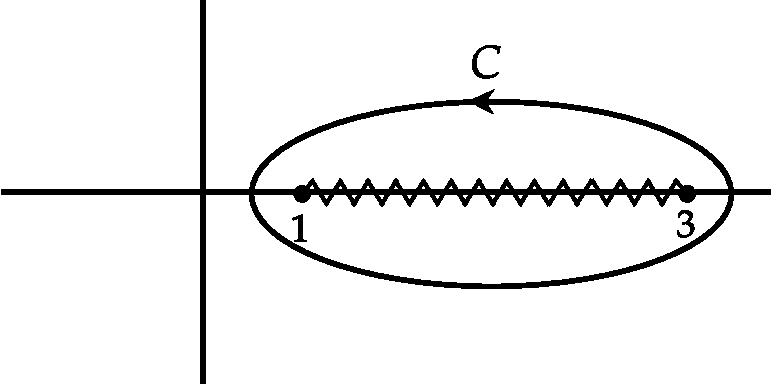
\includegraphics[height=3.5cm,width=6cm]{diagram-20211005(8)-crop}
	\end{figure}
	This integral is equivalent to an integral along the contours
	{\exyear{NET/JRF(DEC-2018)}}
	\begin{tasks}(2)
		\task[\textbf{A.}] \begin{figure}[H]
			\centering
			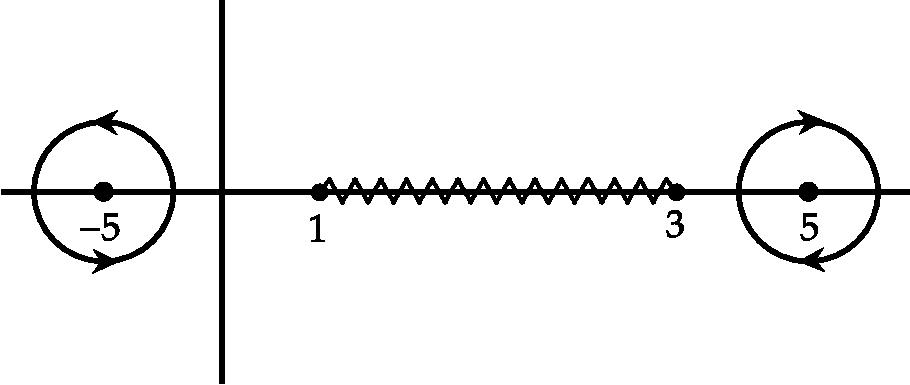
\includegraphics[height=3cm,width=6.5cm]{diagram-20211005(4)-crop}
		\end{figure}
		\task[\textbf{B.}] \begin{figure}[H]
			\centering
			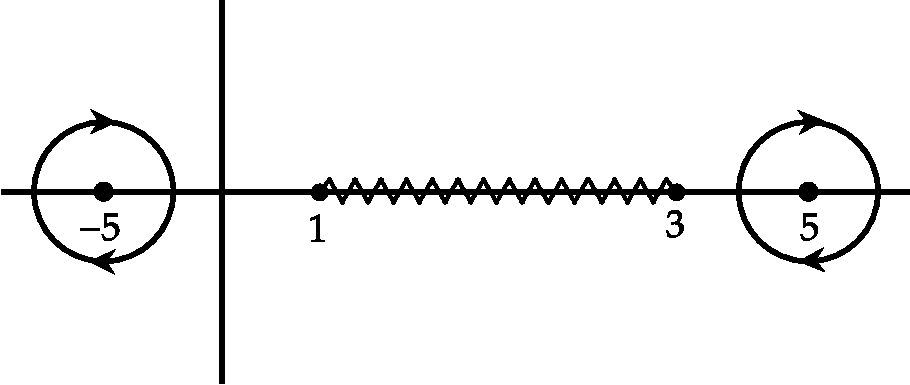
\includegraphics[height=3cm,width=6.5cm]{diagram-20211005(5)-crop}
		\end{figure}
		\task[\textbf{C.}] \begin{figure}[H]
			\centering
			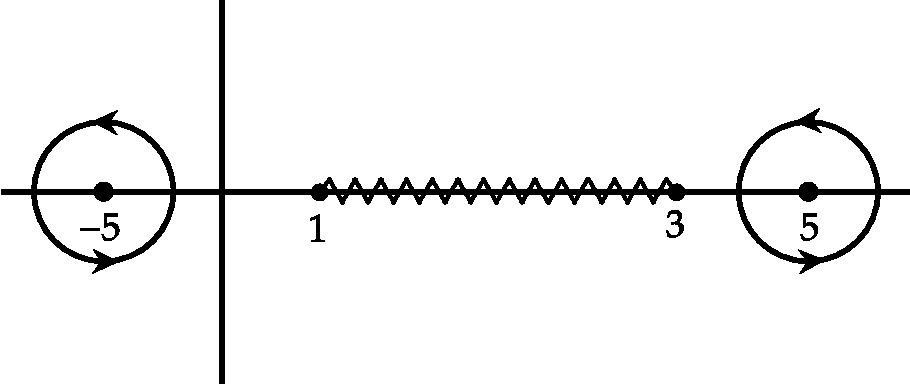
\includegraphics[height=3cm,width=6.5cm]{diagram-20211005(6)-crop}
		\end{figure}
		\task[\textbf{D.}] \begin{figure}[H]
			\centering
			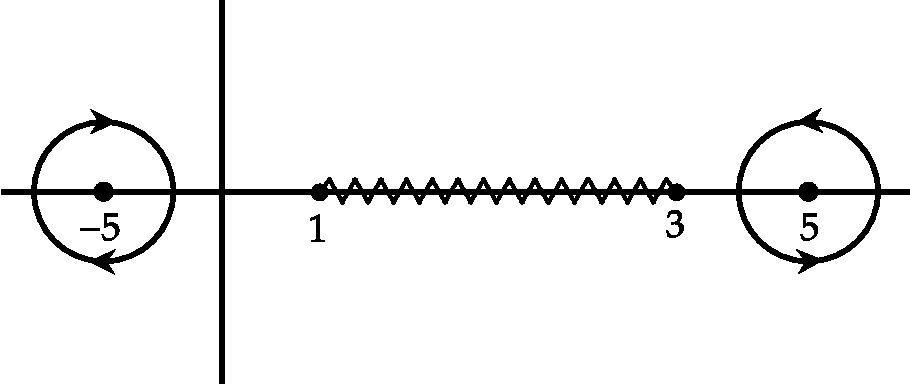
\includegraphics[height=3cm,width=6.5cm]{diagram-20211005(7)-crop}
		\end{figure}
	\end{tasks}
	\begin{answer}
		\begin{align*}
		\intertext{$z=1,3$ are branch points $\infty$ is not a branch point 1 branch cut 3}
		\end{align*}
		So the correct answer is \textbf{Option (C)}
	\end{answer}
	\item  Let $C$ be the circle of radius $\frac{\pi}{4}$ centered at $z=\frac{1}{4}$ in the complex $z$-plane that is traversed counter-clockwise. The value of the contour integral $\oint_{C} \frac{z^{2}}{\sin ^{2} 4 z} d z$ is
	{\exyear{NET/JRF(DEC-2019)}}
	\begin{tasks}(4)
		\task[\textbf{A.}] 0
		\task[\textbf{B.}] $\frac{i \pi^{2}}{4}$
		\task[\textbf{C.}] $\frac{i \pi^{2}}{16}$
		\task[\textbf{D.}] $\frac{i \pi}{4}$
	\end{tasks}
	\begin{answer}$\left. \right. $
		\begin{figure}[H]
			\centering
			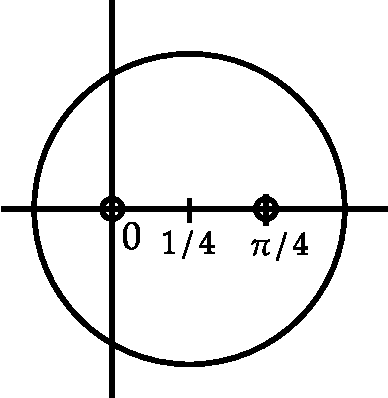
\includegraphics[height=3cm,width=3cm]{diagram-20211026(16)-crop}
		\end{figure}
		\begin{align*}
		f(z)&=\left(\frac{\pi}{\sin 4 z}\right)^{2}\\
		z_{0}&=0, \frac{\pi}{4}\text{ are poles}\\
		4 z&=n \pi, z=0, \frac{\pi}{4}
		\intertext{Others are outside the contour.}
		\text{Residue at }z&=0\text{ is }\left[\frac{\pi}{4 z-\frac{4^{3} z^{3}}{3 !}+\ldots}\right]^{2}\\
		&=\left[\frac{1}{4-\frac{4^{3} z^{2}}{3 !}+\ldots .}\right]^{2}\qquad \text{ No terms for } \frac{1}{z}, b_{1}=0\\
		&=\left[4-\frac{4^{3} z^{2}}{3 !}+\ldots .\right]^{-2}\\
		\text{Residue for }z&=\frac{\pi}{4}\\
		z-\frac{\pi}{4}&=t
		\intertext{$\sin (4 t+\pi)=-\sin 4 t \quad$ (But square so no effect)}
		&\left[\frac{t+\frac{\pi}{4}}{\sin 4\left(t+\frac{\pi}{4}\right)}\right]^{2}\\
		\left(\frac{t+\frac{\pi}{4}}{\sin 4 t}\right)^{2}&=\frac{t^{2}+\frac{\pi^{2}}{4}+2 t \cdot \frac{\pi}{4}}{\sin ^{2} 4 t}\\
		\frac{\pi}{2} \frac{t}{16 t^{2}[1-\ldots .]^{2}}&=\frac{\pi}{32 t}[1-\ldots .]^{-2} \text{(from first term)}\\
		b_{1}&=\frac{\pi}{32}\\
		\oint_{C} \frac{z^{2}}{\sin ^{2} 4 z} d z&=2 \pi i\left[0+\frac{\pi}{32}\right]=\frac{i \pi^{2}}{16}
		\end{align*}
		So the correct answer is \textbf{Option (C)}
	\end{answer}
	\item  A function of a complex variable $z$ is defined by the integral $f(z)=\oint_{\Gamma} \frac{w^{2}-2}{w-z} d w$, where $\Gamma$ is a circular contour of radius 3 , centred at origin, running counter-clockwise in the $w$ - plane. The value of the function at $z=(2-i)$ is
	{\exyear{NET/JRF(JUNE-2020)}}
	\begin{tasks}(4)
		\task[\textbf{A.}] 0
		\task[\textbf{B.}] $1-4 i$
		\task[\textbf{C.}]  $8 \pi+2 \pi \mathrm{i}$
		\task[\textbf{D.}] $-\frac{2}{\pi}-\frac{i}{2 \pi}$
	\end{tasks}
	\begin{answer}$\left. \right. $
		\begin{figure}[H]
			\centering
			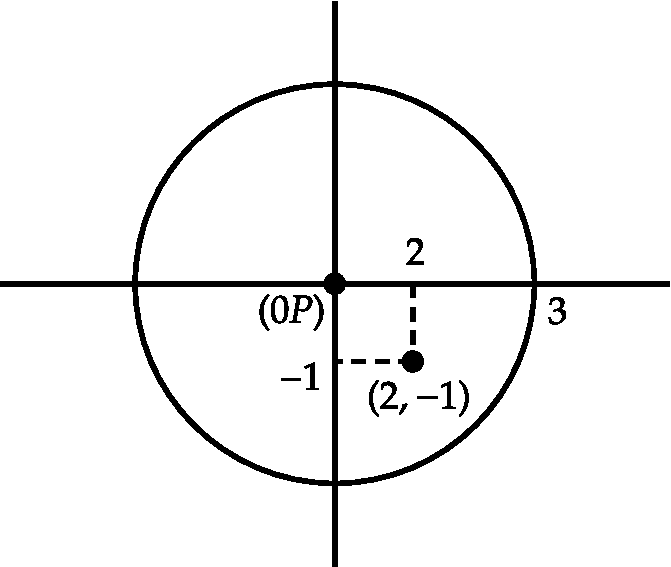
\includegraphics[height=4cm,width=4.6cm]{diagram-20211027-crop}
		\end{figure}
		\begin{align*}
		f(z)&=\oint_{\Gamma} \frac{w^{2}-2}{w-z} d w\\
		\omega&=z\text{ is a simple pole.}\\
		\text{Residue }\lim _{\omega \rightarrow z}(\omega-z) \frac{\left(\omega^{2}-2\right)}{(\omega-z)}&=(2-i)^{2}-2 \\&=4-1-4 i-2=(1-4 i)\\
		f(z)&=\oint_{\Gamma} \frac{w^{2}-2}{w-z} d w=2 \pi i(1-4 i)=2 \pi i+8 \pi
		\end{align*}
		So the correct answer is \textbf{Option (C)}
	\end{answer}
\end{enumerate}
\colorlet{ocre1}{ocre!70!}
\colorlet{ocrel}{ocre!30!}
\setlength\arrayrulewidth{1pt}
\begin{table}[H]
	\centering
	\arrayrulecolor{ocre}
	\begin{tabular}{|p{1.5cm}|p{1.5cm}||p{1.5cm}|p{1.5cm}|}
		\hline
		\multicolumn{4}{|c|}{\textbf{Answer key}}\\\hline\hline
		\rowcolor{ocrel}Q.No.&Answer&Q.No.&Answer\\\hline
		1&\textbf{C} &2&\textbf{B}\\\hline 
		3&\textbf{B} &4&\textbf{A} \\\hline
		5&\textbf{A} &6&\textbf{D} \\\hline
		7&\textbf{A}&8&\textbf{-}\\\hline
		9&\textbf{C}&10&\textbf{A}\\\hline
		11&\textbf{C} &12&\textbf{-}\\\hline
		13&\textbf{A}&14&\textbf{B}\\\hline
		15&\textbf{C}&16&\textbf{B}\\\hline
		17&\textbf{C} &18&\textbf{A}\\\hline
		19&\textbf{B}&20&\textbf{B}\\\hline
		21&\textbf{C}&22&\textbf{C}\\\hline
		23&\textbf{C}& &\\\hline
		
	\end{tabular}
\end{table}
\newpage
\begin{abox}
	Practise Set-2
\end{abox}
\begin{enumerate}[label=\color{ocre}\textbf{\arabic*.}]
	\item  The value of the integral $\oint_{C} \frac{e^{z} \sin (z)}{z^{2}} d z$, where the contour $C$ is the unit circle: $|z-2|=1$, is
	{\exyear{GATE 2010}}
	\begin{tasks}(4)
		\task[\textbf{A.}] $2 \pi i$
		\task[\textbf{B.}] $4 \pi i$
		\task[\textbf{C.}] $\pi i$
		\task[\textbf{D.}] 0
	\end{tasks}
	\begin{answer}
		\begin{align*}
		\intertext{$|z-2|=1 \Rightarrow 1<z<3$ i.e. the pole $z=0$ does not lie inside the contour.}
		\therefore \quad \oint_{C} \frac{e^{z} \sin z}{z^{2}} d z=2 \pi i \times 0=0 .
		\end{align*}
		So the correct answer is \textbf{Option (D)}
	\end{answer}
	\item Which of the following statements is TRUE for the function $f(z)=\frac{z \sin z}{(z-\pi)^{2}}$ ?
	{\exyear{GATE 2011}}
	\begin{tasks}(1)
		\task[\textbf{A.}] $f(z)$ is analytic everywhere in the complex plane
		\task[\textbf{B.}] $f(z)$ has a zero at $z=\pi$
		\task[\textbf{C.}] $f(z)$ has a pole of order 2 at $z=\pi$
		\task[\textbf{D.}] $f(z)$ has a simple pole at $z=\pi$
	\end{tasks}
	\begin{answer}
		\begin{align*}
		f(z)=\frac{z \sin z}{(z-\pi)^{2}}\text{ has a pole of order 2 at }z=\pi
		\end{align*}
		So the correct answer is \textbf{Option (C)}
	\end{answer}
	\item For the function $f(z)=\frac{16 z}{(z+3)(z-1)^{2}}$, the residue at the pole $z=1$ is (your answer should be an integer)-------
	{\exyear{GATE 2013}}
	\begin{answer}
		\begin{align*}
		\text{	At }z&=1,\text{ pole is of order 2 .} \\&\text{So, residue is }\frac{1}{\lfloor-1} \frac{d^{2-1}}{d z^{2-1}}\left[\frac{(z-1)^{2} 16 z}{(z+3)(z-1)^{2}}\right]_{z=1}=3
		\end{align*}
	\end{answer}
	\item The value of the integral
	$$
	\oint_{C} \frac{z^{2}}{e^{z}+1} d z
	$$
	where $C$ is the circle $|z|=4$, is
	{\exyear{GATE 2014}}
	\begin{tasks}(4)
		\task[\textbf{A.}] $2 \pi i$
		\task[\textbf{B.}] $2 \pi^{2} i$
		\task[\textbf{C.}]  $4 \pi^{3} i$
		\task[\textbf{D.}] $4 \pi^{2} i$
	\end{tasks}
	\begin{answer}
		\begin{align*}
		\text{	Pole }e^{z}&=-1 \Rightarrow e^{z}=e^{i(2 m+1) \pi}\text{ where }m=0,1,2,3 \ldots \ldots\\
		\text{For }z&=i \pi,\text{ Res }=\lim _{z=i \pi} \frac{\phi(z)}{\phi^{\prime}(z)}\\&=-\frac{\pi^{2}}{e^{i \pi}}=\pi^{2}\\
		\text{Similarly, for }z&=-i \pi,\text{ Res }=\pi^{2}\\
		\therefore I&=2 \pi i\left(\pi^{2}+\pi^{2}\right)=4 \pi^{3} i
		\end{align*}
			So the correct answer is \textbf{Option (C)}
	\end{answer}
	\item Consider a complex function $f(z)=\frac{1}{z\left(z+\frac{1}{2}\right) \cos (z \pi)}$. Which one of the following statements is correct?
	{\exyear{GATE 2015}}
	\begin{tasks}(1)
		\task[\textbf{A.}] $f(z)$ has simple poles at $z=0$ and $z=-\frac{1}{2}$
		\task[\textbf{B.}] $f(z)$ has second order pole at $z=-\frac{1}{2}$
		\task[\textbf{C.}] $f(z)$ has infinite number of second order poles
		\task[\textbf{D.}] $f(z)$ has all simple poles
	\end{tasks}
	\begin{answer}
		\begin{align*}
		f(z)&=\frac{1}{z\left(z+\frac{1}{2}\right) \cos (z \pi)}\\
		\text{	For $n^{t h}$ order pole, Res. }&=\lim _{z \rightarrow a}(z-a)^{n} f(z)=\text{ finite}\\
		\text{At }z&=0, \lim _{z \rightarrow 0} z f(z)=\text{ finite }\\\Rightarrow z&=0\text{ is a simple pole.}\\
		\text{At }z&=-\frac{1}{2}, \lim _{z \rightarrow-\frac{1}{2}} \frac{\left(z+\frac{1}{2}\right)^{2}}{z\left(z+\frac{1}{2}\right) \cos z \pi}=\lim _{z \rightarrow-\frac{1}{2}} \frac{\left(z+\frac{1}{2}\right)}{z \cos z \pi}\\&=\lim _{z \rightarrow-\frac{1}{2}} \frac{1}{1 . \cos z \pi+z . \pi(-\sin z \pi)}\\
		&=\lim _{z \rightarrow-\frac{1}{2}} \frac{1}{\cos z \pi-z \pi \sin z \pi}=\frac{1}{-\frac{\pi}{2}}\\&=-\frac{2}{\pi}=\text{ finite}\\
		\Rightarrow f(z)\text{ has second order pole at }z&=-\frac{1}{2}
		\end{align*}
		So the correct answer is \textbf{Option (A)}
	\end{answer}
	\item  Consider $w=f(z)=u(x, y)+i v(x, y)$ to be an analytic function in a domain $D$. Which one of the following options is NOT correct?
	{\exyear{GATE 2015}}
	\begin{tasks}(1)
		\task[\textbf{A.}] $u(x, y)$ satisfies Laplace equation in D
		\task[\textbf{B.}]  $v(x, y)$ satisfies Laplace equation in $D$
		\task[\textbf{C.}] $\int_{1}^{z_{2}} f(z) d z$ is dependent on the choice of the contour between $z_{1}$ and $z_{2}$ in $D$
		\task[\textbf{D.}]  $f(z)$ can be Taylor expended in $D$
	\end{tasks}
	\begin{answer}
		\begin{align*}
		w&=f(z)=u(x, y)+i v(x, y)\text{ to be an analytic function in a domain }D, \int_{z_{1}}^{z_{2}} f(z) d z\text{ is}\\
		&\text{independent of the choice of the contour between }z_{1}\text{ and }z_{2}\text{ in }D.
		\end{align*}
		So the correct answer is \textbf{Option (C)}
	\end{answer}
	\item A function $y(z)$ satisfies the ordinary differential equation $y^{\prime \prime}+\frac{1}{z} y^{\prime}-\frac{m^{2}}{z^{2}} y=0$, where\\
	$m=0,1,2,3, \ldots . .$ Consider the four statements P, Q, R, S as given below.\\
	$\mathrm{P}: z^{m}$ and $z^{-m}$ are linearly independent solutions for all values of $m$\\
	Q: $z^{m}$ and $z^{-m}$ are linearly independent solutions for all values of $m>0$\\
	$\mathrm{R}$ : $\ln z$ and 1 are linearly independent solutions for $m=0$\\
	S: $z^{m}$ and $\ln z$ are linearly independent solutions for all values of $m$\\
	The correct option for the combination of valid statements is
	{\exyear{GATE 2015}}
	\begin{tasks}(4)
		\task[\textbf{A.}] P, R and S only
		\task[\textbf{B.}]  P and R only
		\task[\textbf{C.}] $\mathrm{Q}$ and $\mathrm{R}$ only
		\task[\textbf{D.}] $\mathrm{R}$ and $\mathrm{S}$ only
	\end{tasks}
	\begin{answer}
		\begin{align*}
		y^{\prime \prime}+\frac{1}{z} y^{\prime}-\frac{m^{2}}{z^{2}} y&=0 \Rightarrow z^{2} y^{\prime \prime}+z y^{\prime}-m^{2} y\\&=0, m=0,1,2,3, \ldots, \quad z=e^{x}, D=\frac{d}{d x}\\
		\text{	If }m&=0 ; \quad z^{2} y^{\prime \prime}+z y^{\prime}=0,[D(D-1)+D] y\\&=0 \Rightarrow\left[D^{2}-D+D\right] y=0\\
		D^{2} y&=0 \Rightarrow y=c_{1}+c_{2} x \Rightarrow y\\&=c_{1}+c_{2} \ln z \quad \text{( $R$ is correct)}\\
		\text{And if }m &\neq 0, m>0,\text{ then }m \neq 0,\text{ then }\left(D^{2}-m^{2}\right) y\\&=0 \Rightarrow D=\pm m\\
		y&=c_{1} e^{m x}+c_{2} e^{-m x}=c_{1} e^{m \log z}+c_{2} e^{-m \log z}\\&=c_{1} z^{m}+c_{2} z^{-m}\\
		\text{or if }m &\neq 0, m>0,\text{ then}\\
		y&=c_{1} \cosh (m \log (z))+i c_{2} \sinh (m \log (x)), \quad m>0
		\end{align*}
		So the correct answer is \textbf{Option (C)} 
	\end{answer}
	\item  Which of the following is an analytic function of $z$ everywhere in the complex plane?
	{\exyear{GATE 2016}}
	\begin{tasks}(4)
		\task[\textbf{A.}] $z^{2}$
		\task[\textbf{B.}]  $\left(z^{*}\right)^{2}$
		\task[\textbf{C.}] $|z|^{2}$
		\task[\textbf{D.}] $\sqrt{z}$
	\end{tasks}
	\begin{answer}
		\begin{align*}
		z^{2}&=(x+i y)^{2}=x^{2}-y^{2}+i(2 x y) \Rightarrow u\\&=x^{2}-y^{2}\text{ and }v=2 x y\\
		\text{Cauchy Riemann equations }\frac{\partial u}{\partial x}&=\frac{\partial v}{\partial y}=2 x, \quad \frac{\partial v}{\partial x}=-\frac{\partial u}{\partial y}=2 y\text{ satisfies.}
		\end{align*}
		So the correct answer is \textbf{Option (A)}
	\end{answer}
	\item The contour integral $\oint \frac{d z}{1+z^{2}}$ evaluated along a contour going from $-\infty$ to $+\infty$ along the
	real axis and closed in the lower half-plane circle is equal to............... (up to two decimal places).
	{\exyear{GATE 2017}}
	\begin{answer}
		\begin{align*}
		\oint_{c} \frac{1}{1+z^{2}} d z&=\int_{-\infty}^{+\infty} \frac{1}{1+x^{2}} d x+\oint_{c} \frac{1}{1+z^{2}} d z\\
		\text{Poles, }1+z^{2}&=0 \Rightarrow z=\pm i, \quad z=-i\text{ is inside }C\\
		\therefore \operatorname{Res}(z=-i)&=\lim _{z \rightarrow-i}(z+i) \frac{1}{(z-i)(z+i)}\\&=\frac{1}{-i-i}=\frac{1}{-2 i}\\
		\int_{-\infty}^{+\infty} \frac{1}{1+x^{2}} d x&=-\frac{1}{2 i} \times-2 \pi i=\pi
		\intertext{(Since, here we use lower half plane i.e., we traversed in clockwise direction, hence we have to take $-2 \pi i$ )}
		\end{align*}
	\end{answer}
	\item The imaginary part of an analytic complex function is $v(x, y)=2 x y+3 y .$ The real part of the function is zero at the origin. The value of the real part of the function at $1+i$ is ................. (up to two decimal places)
	{\exyear{GATE 2017}}
	\begin{answer}
		\begin{align*}
		\intertext{Solution: The imaginary part of the given analytic function is $v(x, y)=2 x y+3 y .$ From the
			Cauchy - Riemann condition}
		\frac{\partial v}{\partial y}&=\frac{\partial u}{\partial x}=2 x+3
		\intertext{Integrating partially gives}
		u(x, y)&=x^{2}+3 x+g(y)\\
		\intertext{From the second Cauchy - Riemann condition}
		\frac{\partial u}{\partial y}&=-\frac{\partial v}{\partial x},\text{ we obtain} \frac{\partial u}{\partial y}\\&=-2 y, \mu(x, y)=-y^{2}+g(x)\\
		\frac{d g(y)}{d y}&=-2 y \Rightarrow g(y)=-y^{2}+c\\
		\text{	Hence, }u(x, y)&=x^{2}+3 x-y^{2}+c
		\intertext{Since, the real part of the analytic function is zero at the origin.}
		\text{Hence, }0&=0+0-0+c \Rightarrow c=0\\
		\text{Thus, }u(x, y)&=x^{2}+3 x-y^{2}\\
		\therefore f(z)&=\left(x^{2}+3 x-y^{2}\right)+i(2 x y+3 y)
		\intertext{Thus, the value of real part when}
		z&=1+i, i.e. x=1\text{ and }y=1\text{ is }u(x, y)\\&=(1)^{2}+3(1)-1=3
		\end{align*}
	\end{answer}
	\item The absolute value of the integral
	$$
	\int \frac{5 z^{3}+3 z^{2}}{z^{2}-4} d z
	$$
	over the circle $|z-1.5|=1$ in complex plane, is $\ldots$ (up to two decimal places).
	{\exyear{GATE 2018}}
	\begin{answer}
		\begin{align*}
		f(z)&=\frac{5 z^{3}+3 z^{2}}{(z-2)(z+2)}\\
		\text{Pole, }z&=2,-2\\
		z&=-2 \text{ is outside the center}\\
		|-2-1.5|>1&\text{So, will not be considered}\\
		\text{	Now, }\operatorname{Re} s(2)&=\lim _{z \rightarrow 2}(z-2) \frac{\left(5 z^{3}+3 z^{2}\right)}{(z-2)(z+2)}\\&=\frac{52^{3}+32^{2}}{4}=\frac{40+12}{4}=13\\
		I&=2 \pi i \times residue =2 \pi i \times 13\\&=26 \times 3.14 \Rightarrow I=81.64
		\end{align*}
	\end{answer}
	\item The pole of the function $f(z)=\cot z$ at $z=0$ is
	{\exyear{GATE 2019}}
	\begin{tasks}(2)
		\task[\textbf{A.}] A removable pole
		\task[\textbf{B.}] An essential singularity
		\task[\textbf{C.}]  A simple pole
		\task[\textbf{D.}] A second order pole
	\end{tasks}
	\begin{answer}
		\begin{align*}
		f(z)&=\cot z\text{ at }z=0\\
		f(z)&=\frac{1}{\tan z} \quad z=0\text{ is a simple pole }\\f(z)&=\frac{1}{z}\left[1-\frac{1}{3} z^{2}+\ldots .\right]
		\end{align*}
		So the correct answer is \textbf{Option (C)}
	\end{answer}
	\item The value of the integral $\int_{-\infty}^{\infty} \frac{\cos (k x)}{x^{2}+a^{2}} d x$, where $k>0$ and $a>0$, is
	{\exyear{GATE 2019}}
	\begin{tasks}(4)
		\task[\textbf{A.}] $\frac{\pi}{a} e^{-k a}$
		\task[\textbf{B.}] $\frac{2 \pi}{a} e^{-k a}$
		\task[\textbf{C.}] $\frac{\pi}{2 a} e^{-k a}$
		\task[\textbf{D.}] $\frac{3 \pi}{2 a} e^{-k a}$
	\end{tasks}
	\begin{answer}
		\begin{align*}
		&\int_{-\infty}^{\infty} \frac{\cos k x}{x^{2}+a^{2}} d x\\
		f(z)&=\frac{e^{i k x}}{z^{2}+a^{2}}=\frac{e^{i k z}}{(z+i a)(z-i a)}\\
		I&=\operatorname{Re} .2 \pi i \times \frac{e^{i k(i a)}}{2 i a}=\frac{\pi e^{-k a}}{a}
		\end{align*}
		So the correct answer is \textbf{Option (A)}
	\end{answer}
\item The value of the integral $\int_{0}^{\infty} \frac{\ln x}{\left(x^{2}+1\right)^{2}} d x$ is
{\exyear{ JEST 2012}}
 \begin{tasks}(2)
	\task[\textbf{a.}]0
	\task[\textbf{b.}]$\frac{-\pi}{4}$
	\task[\textbf{c.}] $\frac{-\pi}{2}$
	\task[\textbf{d.}] $\frac{\pi}{2}$
\end{tasks}
\begin{answer}$\left. \right. $
	\begin{figure}[H]
		\centering
		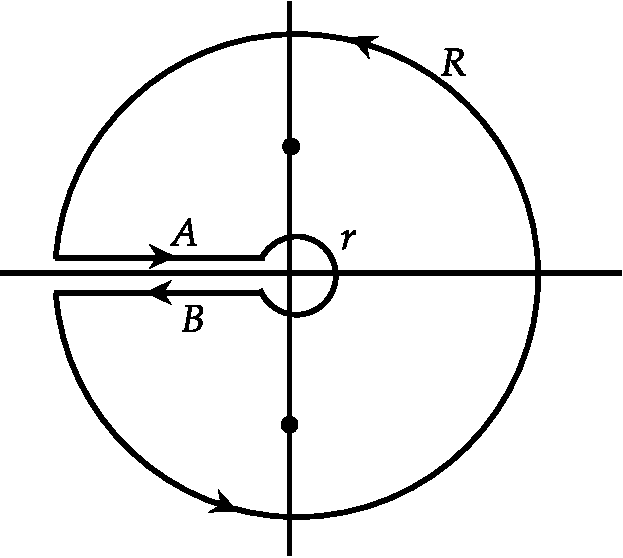
\includegraphics[height=4cm,width=4.6cm]{JEST 01 2012}
	\end{figure}
	\begin{align*}
	\int_{0}^{\infty} \frac{\ln x}{\left(x^{2}+1\right)^{2}} d x&=\int_{0}^{\infty} \frac{\ln z}{\left(z^{2}+1\right)^{2}} d z\\
	\text{Let us consider new function }f(z)&=\left(\frac{\ln z}{z^{2}+1}\right)^{2},\text{ then }I=\int_{0}^{\infty}\left(\frac{\ln z}{z^{2}+1}\right)^{2} d z\\
\text{	Pole at }z&=\pm i\text{ is simple pole of second order.}\\
\text{	Residue at }z&=i\text{ is}\\
&=\frac{d}{d z}(z-i)^{2} \frac{(\ln z)^{2}}{(z-i)^{2}(z+i)^{2}}=\frac{d}{d z} \frac{(\ln z)^{2}}{(z+i)^{2}}\\
&=\frac{(z+i)^{2} 2(\ln z) \cdot \frac{1}{z}-(\ln z)^{2} \cdot 2(z+i)}{(z+i)^{4}}=\frac{(z+i) 2 \ln (z) \frac{1}{z}-(\ln z)^{2} \cdot 2}{(z+i)^{3}}\\
&=\frac{(2 i) 2 \times \frac{1}{i} \ln i-(\ln i)^{2} \cdot 2}{(2 i)^{3}}=\frac{4 \frac{i \pi}{2}-\left(\frac{i \pi}{2}\right)^{2} \times 2}{-8 i}=\frac{2 \pi i+\frac{\pi^{2}}{2}}{-8 i}\\
\left.\Rightarrow \operatorname{Res}\right|_{z=i}&=\frac{-\pi}{4}+\frac{\pi^{2}}{16} i\\
\text{Similarly, at }z&=-i ;\left.\operatorname{Res}\right|_{z=-i}=\frac{-\pi}{4}-\frac{\pi^{2}}{16} i\\
I&=\int_{0}^{\infty}\left(\frac{\ln z}{z^{2}+1}\right)^{2} d z=2 \pi i\left(\frac{-\pi}{4}+\frac{\pi^{2}}{16} i-\frac{\pi}{4}-\frac{\pi^{2}}{16} i\right)=-\pi^{2} i\\
-\pi^{2} i&=\left(\int_{R} \int_{A} \int_{B}\right) f(z) d z=\left(\iint_{A B}\right) f(z) d z ;\qquad \left[\because \int_{A B}\right.\text{ vanish }]\\
\text{Along path }A ;& \quad z=-x+i \varepsilon\text{ and along path }B ; \quad z=-x-i \varepsilon\\
\text{Thus }-\pi^{2} i&=\left(\iint_{A B}\right) f(z) d z=-\int_{-\infty}^{0}\left[\frac{\ln (-x+i \varepsilon)}{(-x+i \varepsilon)^{2}+1}\right] d x-\int_{0}^{\infty}\left[\frac{\ln (-x-i \varepsilon)}{(-x-i \varepsilon)^{2}+1}\right] d x\\
\Rightarrow-\pi^{2} i&=\int_{0}^{\infty}\left[\frac{\ln (-x+i \varepsilon)}{(-x+i \varepsilon)^{2}+1}\right]^{2} d x-\int_{0}^{\infty}\left[\frac{\ln (-x-i \varepsilon)}{(-x-i \varepsilon)^{2}+1}\right]^{2} d x\\
\Rightarrow-\pi^{2} i&=\int_{0}^{\infty}\left[\frac{\ln (x)+i \pi}{1+x^{2}}\right]^{2} d x-\int_{0}^{\infty}\left[\frac{\ln (x)-i \pi}{1+x^{2}}\right]^{2} d x ; \quad \varepsilon \rightarrow 0\\
\Rightarrow-\pi^{2} i&=\int_{0}^{\infty} \frac{(\ln (x)+i \pi)^{2}-(\ln (x)-i \pi)^{2}}{\left(1+x^{2}\right)^{2}} d x\\&=4 \pi i \int_{0}^{\infty} \frac{\ln x}{\left(x^{2}+1\right)^{2}} \Rightarrow \int_{0}^{\infty} \frac{\ln x}{\left(x^{2}+1\right)^{2}}=\frac{-i \pi^{2}}{4 \pi i}=\frac{-\pi}{4}
	\end{align*}
		So the correct answer is \textbf{Option (B)}
\end{answer}
\item Compute $\lim _{z \rightarrow 0} \frac{\operatorname{Re}\left(z^{2}\right)+\operatorname{Im}\left(z^{2}\right)}{z^{2}}$
{\exyear{ JEST 2013}}
 \begin{tasks}(2)
	\task[\textbf{a.}] The limit does not exist
	\task[\textbf{b.}]1
	\task[\textbf{c.}]$-i$
	\task[\textbf{d.}] $-1$
\end{tasks}
\begin{answer}
	\begin{align*}
	\lim _{z \rightarrow 0} \frac{\operatorname{Re}\left(z^{2}\right)+\operatorname{Im}\left(z^{2}\right)}{z^{2}}&=\lim _{z \rightarrow 0} \frac{x^{2}-y^{2}+2 x y}{x^{2}-y^{2}+2 i x y}=\lim _{y=0 \atop x \rightarrow 0} \frac{x^{2}-y^{2}+2 x y}{x^{2}-y^{2}+2 i x y}=1\\
	\lim _{x=0 \atop y \rightarrow 0} \frac{x^{2}-y^{2}+2 x y}{x^{2}-y^{2}+2 i x y}&=1\text{ and }\lim _{y=x \atop x \rightarrow 0} \frac{x^{2}-y^{2}+2 x y}{x^{2}-y^{2}+2 i x y}=-i
	\end{align*}
		So the correct answer is \textbf{Option (A)}
\end{answer}
\item The value of limit
$$
\lim _{z \rightarrow i} \frac{z^{10}+1}{z^{6}+1}
$$
is equal to
{\exyear{ JEST 2014}}
 \begin{tasks}(2)
	\task[\textbf{a.}]1
	\task[\textbf{b.}]0
	\task[\textbf{c.}] $\frac{-10}{3}$
	\task[\textbf{d.}] $\frac{5}{3}$
\end{tasks}
\begin{answer}
	\begin{align*}
	\lim _{z \rightarrow i} \frac{z^{10}+1}{z^{6}+1}=\lim _{z \rightarrow i} \frac{10 z^{9}}{6 z^{5}}=\lim _{z \rightarrow i} \frac{10 z^{4}}{6}=\frac{10}{6}=\frac{5}{3}
	\end{align*}
		So the correct answer is \textbf{Option (D)}
\end{answer}
\item The value of integral
$$
I=\oint \frac{\sin z}{2 z-\pi} d z
$$
with $c$ a circle $|z|=2$, is
{\exyear{ JEST 2014}}
 \begin{tasks}(2)
	\task[\textbf{a.}] 0
	\task[\textbf{b.}]$2 \pi i$
	\task[\textbf{c.}] $\pi i$
	\task[\textbf{d.}]  $-\pi i$
\end{tasks}
\begin{answer}
	\begin{align*}
	I&=\oint_{C} \frac{\sin z}{2 z-\pi},\text{ for pole }2 z-\pi=0 \Rightarrow z=\frac{\pi}{2}\\
\text{	Residue at }z&=\frac{\pi}{2}
	\because|z|=2\text{, so pole will lie within the contour}\\
	I&=\oint_{C} \frac{e^{i z}}{2\left(z-\frac{\pi}{2}\right)}=\sum R \times 2 \pi i\\
	\left.\operatorname{Res}\right|_{z=\frac{\pi}{2}}&=\frac{\left(z-\frac{\pi}{2}\right) e^{i z}}{2\left(z-\frac{\pi}{2}\right)}=\frac{e^{i \pi / 2}}{2}=\frac{i}{2}\text{ (taking imaginary part); Residue }=\frac{1}{2}\\
	\text{Now, }I&=\frac{1}{2} \times 2 \pi i=\pi i
	\end{align*}
		So the correct answer is \textbf{Option (C)}
\end{answer}
\item Given an analytic function $f(z)=\phi(x, y)+i \psi(x, y)$, where $\phi(x, y)=x^{2}+4 x-y^{2}+2 y$
If $C$ is a constant, which of the following relations is true?
{\exyear{ JEST 2015}}
 \begin{tasks}(2)
	\task[\textbf{a.}]$\psi(x, y)=x^{2} y+4 y+C$
	\task[\textbf{b.}]$\psi(x, y)=2 x y-2 x+C$
	\task[\textbf{c.}]$\psi(x, y)=2 x y+4 y-2 x+C$
	\task[\textbf{d.}] $\psi(x, y)=x^{2} y-2 x+C$
\end{tasks}
\begin{answer}
	\begin{align}
	u&=\phi(x, y)=x^{2}+4 x-y^{2}+2 y, v=\psi\notag\\
	\text{From C.R. equation, }\frac{\partial u}{\partial x}&=\frac{\partial v}{\partial y}, \Rightarrow \frac{\partial \phi}{\partial x}=\frac{\partial \psi}{\partial y}, \frac{\partial u}{\partial y}=-\frac{\partial v}{\partial x} \Rightarrow \frac{\partial \phi}{\partial y}=-\frac{\partial \psi}{\partial x}\notag\\
	\text{Now, }\frac{\partial \phi}{\partial x}&=2 x+4=\frac{\partial \psi}{\partial y}\notag\\
	\Rightarrow \psi&=2 x y+4 y+f(x)\label{CN 01}\\
	\text{and }\frac{\partial \phi}{\partial y}&=-2 y+2 \Rightarrow \frac{\partial \psi}{\partial x}=+2 y-2\notag\\
	\psi&=2 x y+2 x+f(y)\label{CN 02}\\
	\text{From (\ref{CN 01}) and (\ref{CN 02}), }&2 x y+4 y+f(x)=2 x y-2 x+f(y)\notag\\
	f(x)&=-2 x, \quad f(y)=4 y \notag\\
	\psi&=2 x y+4 y-2 x+c\notag
	\end{align}
		So the correct answer is \textbf{Option (C)}
\end{answer}
\item Which one is the image of the complex domain $\{z \mid x y \geq 1, x+y>0\}$ under the mapping $f(z)=z^{2}$, if $z=x+i y ?$
{\exyear{ JEST 2017}}
 \begin{tasks}(2)
	\task[\textbf{a.}] $\{z \mid x y \geq 1, x+y>0\}$
	\task[\textbf{b.}]$\{z \mid x \geq 2, x+y>0\}$
	\task[\textbf{c.}]$\{z \mid y \geq 2 \forall x\}$
	\task[\textbf{d.}] $\{z \mid y \geq 1 \forall x\}$
\end{tasks}
\item The integral $I=\int_{1}^{\infty} \frac{\sqrt{x-1}}{(1+x)^{2}} d x$ is
{\exyear{ JEST 2017}}
 \begin{tasks}(2)
	\task[\textbf{a.}]$\frac{\pi}{\sqrt{2}}$
	\task[\textbf{b.}]$\frac{\pi}{2 \sqrt{2}}$
	\task[\textbf{c.}]$\frac{\sqrt{\pi}}{2}$
	\task[\textbf{d.}]$\sqrt{\frac{\pi}{2}}$
\end{tasks}
\begin{answer}
	\begin{align*}
	I&=\int_{1}^{\infty} \frac{\sqrt{x-1}}{(1+x)^{2}} d x\\
\text{	Put,} x&=\left(1+z^{2}\right), d x=2 z d z\\
	\text{Hence, }I&=\int_{0}^{\infty} \frac{2 z^{2} d z}{\left(2+z^{2}\right)^{2}}\\
	\text{Here poles, }\left(2+z^{2}\right)&=0 \Rightarrow(z+i \sqrt{2})(z-i \sqrt{2})=0\\
\text{	Only }&(z=i \sqrt{2})\text{ poles is allowed}\\
\text{Then }R(i \sqrt{2})&=\lim _{z \rightarrow i \sqrt{2}} \frac{1}{\sqrt{2-1}} \frac{d}{d z}\left[\frac{2 z^{2}(z-i \sqrt{2})^{2}}{(z-i \sqrt{2})^{2}(z+i \sqrt{2})^{2}}\right]\\
&=\lim _{z \rightarrow i \sqrt{2}}\left[\frac{(z+i \sqrt{2})^{2} \cdot 4 z-2 z^{2} \cdot 2(z+i \sqrt{2})}{(z+i \sqrt{2})^{4}}\right]\\
&=\frac{(2 i \sqrt{2})^{2} \times 4(i \sqrt{2})-2(i \sqrt{2})^{2} \cdot 2(2 i \sqrt{2})}{(2 i \sqrt{2})^{4}}\\&=-\frac{32 \sqrt{2} i+16 \sqrt{2} i}{64}=-\frac{16 \sqrt{2} i}{64}=-\frac{i}{2 \sqrt{2}}\\
\text{Hence, }\int_{-\infty}^{\infty} \frac{2 z^{2}}{\left(2+z^{2}\right)^{2}} d z&=2 \pi i\left(-\frac{i}{2 \sqrt{2}}\right)=\frac{\pi}{\sqrt{2}}\\
\Rightarrow \int_{0}^{\infty} \frac{2 z^{2}}{\left(2+z^{2}\right)^{2}} d z&=\frac{\pi}{2 \sqrt{2}} \Rightarrow \int_{i}^{\infty} \frac{\sqrt{x-1}}{(1+x)^{2}} d x=\frac{\pi}{2 \sqrt{2}}
	\end{align*}
	So the correct answer is \textbf{Option (B)}
\end{answer}
\item The integral
$$
\int_{-\infty}^{\infty} \frac{\cos x}{x^{2}+1} d x \text { is }
$$
{\exyear{ JEST 2018}}
 \begin{tasks}(2)
	\task[\textbf{a.}]$\frac{\pi}{e}$
	\task[\textbf{b.}] $\pi e^{-2}$
	\task[\textbf{c.}]$\pi$
	\task[\textbf{d.}] zero
\end{tasks}
\begin{answer}
	\begin{align*}
	f(z)&=\frac{e^{i z}}{z^{2}+1}=\frac{e^{i z}}{(z+i)(z-i)}\\
	\int_{-\infty}^{\infty} \frac{\cos x}{x^{2}+1} d x&=\operatorname{Re} 2 \pi i \times \frac{e^{i \cdot i}}{z i}=\frac{\pi}{e}
	\end{align*}
		So the correct answer is \textbf{Option (A)}
\end{answer}
\item Consider the function $f(x, y)=|x|-i|y| .$ In which domain of the complex plane is this function analytic?
{\exyear{ JEST 2019}}
 \begin{tasks}(2)
	\task[\textbf{a.}]First and second quadrants
	\task[\textbf{b.}]Second and third quadrants
	\task[\textbf{c.}]Second and fourth quadrants
	\task[\textbf{d.}]  Nowhere
\end{tasks}
\begin{answer}
	\begin{align*}
	 f(x, y)&=|x|-i|y|\\
	f(x, y)&=x-i y=\bar{z}\\
	f(x, y)&=-x-i y=-z\\
	f(x, y)&=-x+i y=-\bar{z}\\
	f(x, y)&=x+i y=z
	\intertext{We know $\bar{z}$ is not analytic and $z$ and $-z$ are analytic. }
	\end{align*}
	So the correct answer is \textbf{Option (C)}
\end{answer}
\end{enumerate}
 \colorlet{ocre1}{ocre!70!}
\colorlet{ocrel}{ocre!30!}
\setlength\arrayrulewidth{1pt}
\begin{table}[H]
	\centering
	\arrayrulecolor{ocre}
	\begin{tabular}{|p{1.5cm}|p{1.7cm}||p{1.5cm}|p{1.5cm}|}
		\hline
		\multicolumn{4}{|c|}{\textbf{Answer key}}\\\hline\hline
		\rowcolor{ocrel}Q.No.&Answer&Q.No.&Answer\\\hline
		1&\textbf{D} &2&\textbf{C}\\\hline 
		3&\textbf{3(NAT)} &4&\textbf{C} \\\hline
		5&\textbf{A} &6&\textbf{C} \\\hline
		7&\textbf{C}&8&\textbf{A}\\\hline
		9&\textbf{$\pi$(NAT)}&10&\textbf{3(NAT)}\\\hline
		11&\textbf{81.64(NAT)} &12&\textbf{C}\\\hline
		13&\textbf{A}& 14&\textbf{B}\\\hline
		15&\textbf{A}&16 &\textbf{D}\\\hline
		17&\textbf{C}&18&\textbf{C}\\\hline
		19&\textbf{-} &20&\textbf{B}\\\hline
		21&\textbf{A}&22&\textbf{C}\\\hline
	\end{tabular}
\end{table}